\section{Write-Back Module}

\begin{figure}[h!]
    \centering
    \vspace{1em}
\scalebox{0.85}{
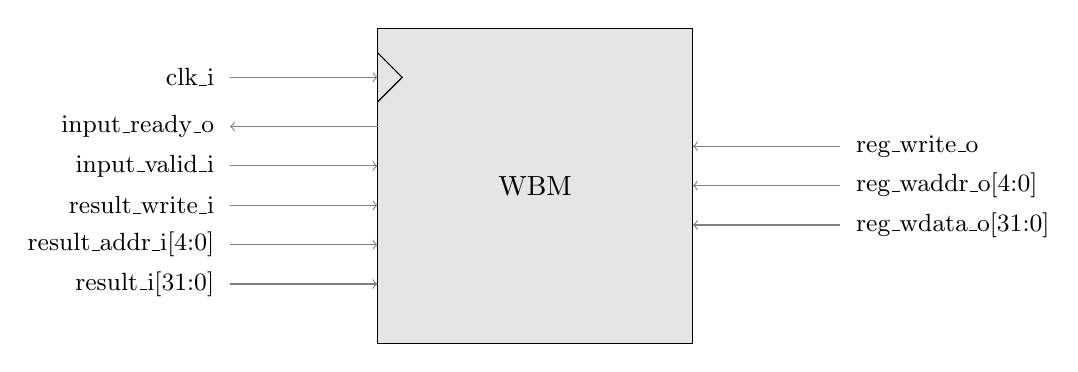
\begin{tikzpicture}[scale=1.25, draw=gray, inner sep=0, outer sep=0]
  \node[rectangle, draw=black,
    anchor=south,
    align=center,
    minimum height = 4cm,
    minimum width = 4cm,
    fill = gray!20] (block) at (0, 0) {WBM};

  \node (rport2) at (block.east) {};
  \node (rport1) at ([yshift=0.4cm]rport2.center) {};
  \node (rport3) at ([yshift=-0.4cm]rport2.center) {};
  \draw[->] ([xshift=1.5cm]rport1.center) node[right=0.2cm, anchor=west]{\small reg\_write\_o} -- (rport1.center);
  \draw[->] ([xshift=1.5cm]rport2.center) node[right=0.2cm, anchor=west]{\small reg\_waddr\_o[4:0]} -- (rport2.center);
  \draw[->] ([xshift=1.5cm]rport3.center) node[right=0.2cm, anchor=west]{\small reg\_wdata\_o[31:0]} -- (rport3.center);

  \node (lport3) at ([yshift=-0.2cm] block.west) {};
  \node (lport2) at ([yshift=0.4cm]lport3.center) {};
  \node (lport1) at ([yshift=0.4cm]lport2.center) {};
  \node (lport4) at ([yshift=-0.4cm]lport3.center) {};
  \node (lport5) at ([yshift=-0.4cm]lport4.center) {};

  \draw[<-] ([xshift=-1.5cm]lport1.center) node[left=0.2cm, anchor=east]{\small input\_ready\_o} -- (lport1.center);
  \draw[->] ([xshift=-1.5cm]lport2.center) node[left=0.2cm, anchor=east]{\small input\_valid\_i} -- (lport2.center);
  \draw[->] ([xshift=-1.5cm]lport3.center) node[left=0.2cm, anchor=east]{\small result\_write\_i} -- (lport3.center);
  \draw[->] ([xshift=-1.5cm]lport4.center) node[left=0.2cm, anchor=east]{\small result\_addr\_i[4:0]} -- (lport4.center);
  \draw[->] ([xshift=-1.5cm]lport5.center) node[left=0.2cm, anchor=east]{\small result\_i[31:0]} -- (lport5.center);

  \node (clk) at ([yshift=-0.5cm]block.north west) {};
  \draw[->] ([xshift=-1.5cm]lport3.center |- clk.center) node[left=0.2cm, anchor=east]{\small clk\_i} -- (clk.center);
  % clk triangle
  \draw[-  , draw=black] ([yshift=0.25cm]clk.center) -- ([xshift=0.25cm]clk.center) -- ([yshift=-0.25cm]clk.center);
\end{tikzpicture}
}

    \caption{Schematic view of the Write-Back Module}
    \label{fig:wbm}
\end{figure}

\subsection{Interface}

\begin{content}
The write-back module implements TBC. The signals are described in table \ref{tab:wbm-interface}. 
\end{content}

\input{arch/tables/wbm-interface}

\subsection{Specification}

\subsubsection{Upstream requirements}

The table \ref{tab:wbm-upstream-requirements} outlines the upstream requirements applicable to the Write-Back Module.

{
  \vspace{0.5em}
  \begin{center}
    \refstepcounter{table}
    Table \thetable: Upstream requirements applicable to the Write-Back Module\label{tab:wbm-upstream-requirements}
  \end{center}
  
\footnotesize
\begin{xltabular}{0.9\textwidth}{|X|c|}
  \hline
  \cellcolor{gray!20}\textbf{ID} \\
  \hline
  \reqref{F\_INSTR\_RESULT\_02} \\
  \hline
\end{xltabular}
}


\subsubsection{Functional requirements}

\req{D\_WBM\_INPUT\_HANDSHAKE\_01}{
  The inputs to the write-back module shall be registered on the rising edge of \texttt{clk\_i} when both \texttt{input\_ready\_o} and \texttt{input\_valid\_i} are asserted.
}

\req{D\_WBM\_WRITE\_REQUEST\_01}{
  The write-back module shall emit a register write request on the rising edge of \texttt{clk\_i} upon registration of its inputs, when \texttt{result\_write\_i} is asserted.
}[
  derivedfrom=F\_INSTR\_RESULT\_02
]

\req{D\_WBM\_WRITE\_REQUEST\_02}{
  The \texttt{reg\_write\_o} signal shall be asserted on the rising edge of \texttt{clk\_i} when emitting a register write request.
}[
  derivedfrom=F\_INSTR\_RESULT\_02
]

\req{D\_WBM\_WRITE\_REQUEST\_03}{
  The \texttt{reg\_waddr\_o} signal shall be set to the registered \texttt{result\_addr\_i} when emitting a register write request.
}[
  derivedfrom=F\_INSTR\_RESULT\_02
]

\req{D\_WBM\_WRITE\_REQUEST\_04}{
  The \texttt{reg\_wdata\_o} signal shall be set to the registered \texttt{result\_i} when emitting a register write request.
}[
  derivedfrom=F\_INSTR\_RESULT\_02
]

\subsection{Behavior}

\subsubsection{Instruction with output behavior}

\begin{content}
  TBC : reg port directly wired to stage ff
\end{content}

\begin{figure}[H]
    \centering
    \makeatletter\gdef\dividers{}
\begin{tikztimingtable}[%
    scale=0.7,
    timing/dslope=0.1,
    timing/.style={x=6ex,y=3ex},
    x=6ex,
    timing/rowdist=4ex,
    timing/name/.style={font=\footnotesize},
    timing/u/background/.style={fill=gray!20},
    timing/e/background/.style={fill=gray!20},
]
clk\_i & H 2{C C} L \\
& \divider{Stage inputs} \\
input\_ready\_o & 2E 2H 2E \\
input\_valid\_i & 2E 2H 2E \\
result\_write\_i & 2E 2H 2E \\
result\_addr\_i[4:0] & 2U 2D 2U \\
result\_data\_i[31:0] & 2U 2D 2U \\
& \divider{Register access} \\
reg\_write\_o & 2E 2H 2E \\
reg\_waddr\_o[4:0] & 2U 2D{result\_addr\_i} 2U \\
reg\_wdata\_o[31:0] & 2U 2D{result\_data\_i} 2U \\
\extracode
% grid
\begin{pgfonlayer}{background}
\begin{scope}[semitransparent ,semithick]
\vertlines[darkgray,dotted]{2, 4}
\dividers
\end{scope}
\end{pgfonlayer}
\end{tikztimingtable}

    \caption{Timing diagram of the instruction with output behavior of the write-back module}
    \label{fig:wbm-behavior-instruction-with-output}
\end{figure}

\subsubsection{Instruction without output behavior}

\begin{content}
  TBC : reg port directly wired to stage ff
\end{content}

\begin{figure}[H]
    \centering
    \makeatletter\gdef\dividers{}
\begin{tikztimingtable}[%
    scale=0.7,
    timing/dslope=0.1,
    timing/.style={x=6ex,y=3ex},
    x=6ex,
    timing/rowdist=4ex,
    timing/name/.style={font=\footnotesize},
    timing/u/background/.style={fill=gray!20},
    timing/e/background/.style={fill=gray!20},
]
clk\_i & H 2{C C} L \\
& \divider{Stage inputs} \\
input\_ready\_o & 2E 2H 2E \\
input\_valid\_i & 2E 2H 2E \\
result\_write\_i & 2E 2L 2E \\
& \divider{Register access} \\
reg\_write\_o & 2E 2L 2E \\
\extracode
% grid
\begin{pgfonlayer}{background}
\begin{scope}[semitransparent ,semithick]
\vertlines[darkgray,dotted]{2, 4}
\dividers
\end{scope}
\end{pgfonlayer}
\end{tikztimingtable}

    \caption{Timing diagram of the instruction without output behavior of the write-back module}
    \label{fig:wbm-behavior-instruction-without-output}
\end{figure}

\subsubsection{Hazard behaviors}

\begin{content}
  Hazard behaviors are described in section \ref{pipeline-stall}.
\end{content}

\newpage
